\documentclass{standalone}
\usepackage{tikz}
\usetikzlibrary{patterns, positioning}


\begin{document}
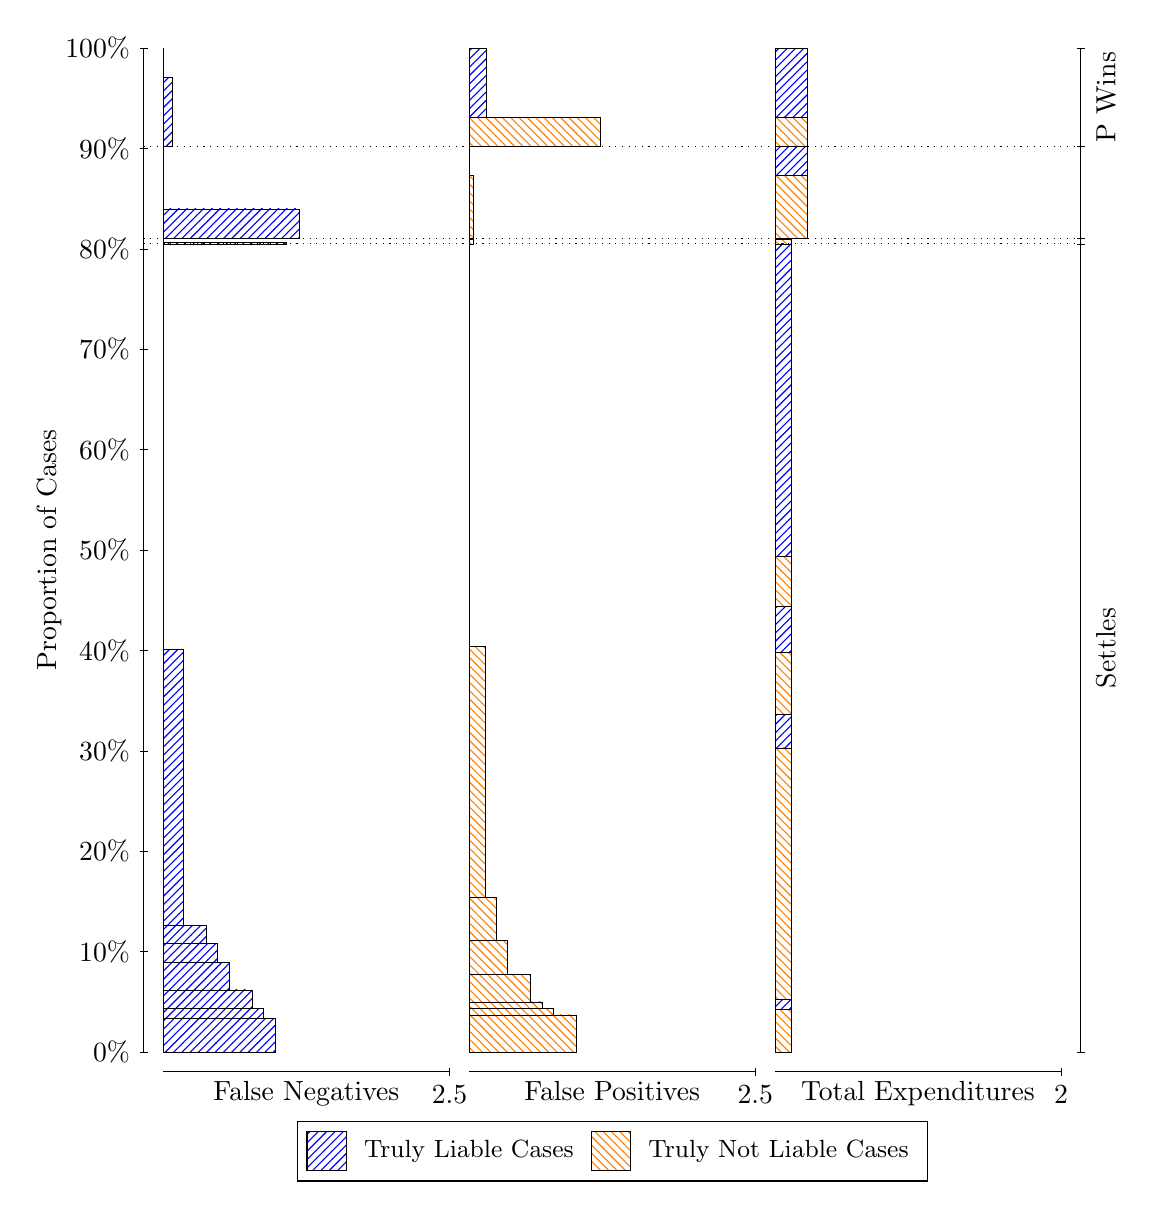
\begin{tikzpicture}
\draw[black, very thin] (1.5,1.75) -- (1.5,14.5);
\node[rotate=90, text=black, anchor=center] at (0.3, 8.125) {Proportion of Cases};
\draw[black, very thin] (1.45,1.75) -- (1.55,1.75);
\node[text=black, anchor=east] at (1.45, 1.75) {0\%};
\draw[black, very thin] (1.45,3.025) -- (1.55,3.025);
\node[text=black, anchor=east] at (1.45, 3.025) {10\%};
\draw[black, very thin] (1.45,4.3) -- (1.55,4.3);
\node[text=black, anchor=east] at (1.45, 4.3) {20\%};
\draw[black, very thin] (1.45,5.575) -- (1.55,5.575);
\node[text=black, anchor=east] at (1.45, 5.575) {30\%};
\draw[black, very thin] (1.45,6.85) -- (1.55,6.85);
\node[text=black, anchor=east] at (1.45, 6.85) {40\%};
\draw[black, very thin] (1.45,8.125) -- (1.55,8.125);
\node[text=black, anchor=east] at (1.45, 8.125) {50\%};
\draw[black, very thin] (1.45,9.4) -- (1.55,9.4);
\node[text=black, anchor=east] at (1.45, 9.4) {60\%};
\draw[black, very thin] (1.45,10.675) -- (1.55,10.675);
\node[text=black, anchor=east] at (1.45, 10.675) {70\%};
\draw[black, very thin] (1.45,11.95) -- (1.55,11.95);
\node[text=black, anchor=east] at (1.45, 11.95) {80\%};
\draw[black, very thin] (1.45,13.225) -- (1.55,13.225);
\node[text=black, anchor=east] at (1.45, 13.225) {90\%};
\draw[black, very thin] (1.45,14.5) -- (1.55,14.5);
\node[text=black, anchor=east] at (1.45, 14.5) {100\%};

\draw[black, very thin] (13.4,1.75) -- (13.4,14.5);
\draw[black, very thin] (13.35,1.75) -- (13.45,1.75);
\node[anchor=west] at (13.35, 1.75) {};
\draw[black, very thin] (13.35,12.012) -- (13.45,12.012);
\node[anchor=west] at (13.35, 12.012) {};
\draw[black, very thin] (13.35,12.085) -- (13.45,12.085);
\node[anchor=west] at (13.35, 12.085) {};
\draw[black, very thin] (13.35,13.25) -- (13.45,13.25);
\node[anchor=west] at (13.35, 13.25) {};
\draw[black, very thin] (13.35,14.5) -- (13.45,14.5);
\node[anchor=west] at (13.35, 14.5) {};

\draw[black, very thin, pattern color=blue, pattern=north east lines] (1.75,1.75) rectangle (3.167,2.1725);
\draw[black, very thin, pattern color=blue, pattern=north east lines] (1.75,2.1725) rectangle (3.0217,2.3031);
\draw[black, very thin, pattern color=blue, pattern=north east lines] (1.75,2.3031) rectangle (2.8763,2.5377);
\draw[black, very thin, pattern color=blue, pattern=north east lines] (1.75,2.5377) rectangle (2.5857,2.8921);
\draw[black, very thin, pattern color=blue, pattern=north east lines] (1.75,2.8921) rectangle (2.4403,3.1263);
\draw[black, very thin, pattern color=blue, pattern=north east lines] (1.75,3.1263) rectangle (2.295,3.3606);
\draw[black, very thin, pattern color=blue, pattern=north east lines] (1.75,3.3606) rectangle (2.0043,6.8586);
\draw[black, very thin, pattern color=orange, pattern=north west lines] (1.75,6.8586) rectangle (1.75,12.012);
\draw[black, very thin, pattern color=blue, pattern=north east lines] (1.75,12.012) rectangle (3.3123,12.029);
\draw[black, very thin, pattern color=orange, pattern=north west lines] (1.75,12.029) rectangle (1.75,12.085);
\draw[black, very thin, pattern color=blue, pattern=north east lines] (1.75,12.085) rectangle (3.4758,12.456);
\draw[black, very thin, pattern color=orange, pattern=north west lines] (1.75,12.456) rectangle (1.75,13.25);
\draw[black, very thin, pattern color=blue, pattern=north east lines] (1.75,13.25) rectangle (1.859,14.128);
\draw[black, very thin, pattern color=orange, pattern=north west lines] (1.75,14.128) rectangle (1.75,14.5);
\draw[black, very thin, pattern color=orange, pattern=north west lines] (5.6333,1.75) rectangle (6.9958,2.2209);
\draw[black, very thin, pattern color=orange, pattern=north west lines] (5.6333,2.2209) rectangle (6.7052,2.3031);
\draw[black, very thin, pattern color=orange, pattern=north west lines] (5.6333,2.3031) rectangle (6.5598,2.3852);
\draw[black, very thin, pattern color=orange, pattern=north west lines] (5.6333,2.3852) rectangle (6.4145,2.7396);
\draw[black, very thin, pattern color=orange, pattern=north west lines] (5.6333,2.7396) rectangle (6.1238,3.1715);
\draw[black, very thin, pattern color=orange, pattern=north west lines] (5.6333,3.1715) rectangle (5.9785,3.7115);
\draw[black, very thin, pattern color=orange, pattern=north west lines] (5.6333,3.7115) rectangle (5.8332,6.9039);
\draw[black, very thin, pattern color=blue, pattern=north east lines] (5.6333,6.9039) rectangle (5.6333,12.012);
\draw[black, very thin, pattern color=orange, pattern=north west lines] (5.6333,12.012) rectangle (5.6878,12.068);
\draw[black, very thin, pattern color=blue, pattern=north east lines] (5.6333,12.068) rectangle (5.6333,12.085);
\draw[black, very thin, pattern color=orange, pattern=north west lines] (5.6333,12.085) rectangle (5.6878,12.878);
\draw[black, very thin, pattern color=blue, pattern=north east lines] (5.6333,12.878) rectangle (5.6333,13.25);
\draw[black, very thin, pattern color=orange, pattern=north west lines] (5.6333,13.25) rectangle (7.3047,13.622);
\draw[black, very thin, pattern color=blue, pattern=north east lines] (5.6333,13.622) rectangle (5.8513,14.5);
\draw[black, very thin, pattern color=orange, pattern=north west lines] (9.5167,1.75) rectangle (9.721,2.29);
\draw[black, very thin, pattern color=blue, pattern=north east lines] (9.5167,2.29) rectangle (9.721,2.4206);
\draw[black, very thin, pattern color=orange, pattern=north west lines] (9.5167,2.4206) rectangle (9.721,5.6129);
\draw[black, very thin, pattern color=blue, pattern=north east lines] (9.5167,5.6129) rectangle (9.721,6.0355);
\draw[black, very thin, pattern color=orange, pattern=north west lines] (9.5167,6.0355) rectangle (9.721,6.8217);
\draw[black, very thin, pattern color=blue, pattern=north east lines] (9.5167,6.8217) rectangle (9.721,7.4107);
\draw[black, very thin, pattern color=orange, pattern=north west lines] (9.5167,7.4107) rectangle (9.721,8.0459);
\draw[black, very thin, pattern color=blue, pattern=north east lines] (9.5167,8.0459) rectangle (9.721,12.012);
\draw[black, very thin, pattern color=orange, pattern=north west lines] (9.5167,12.012) rectangle (9.721,12.068);
\draw[black, very thin, pattern color=blue, pattern=north east lines] (9.5167,12.068) rectangle (9.721,12.085);
\draw[black, very thin, pattern color=orange, pattern=north west lines] (9.5167,12.085) rectangle (9.9254,12.878);
\draw[black, very thin, pattern color=blue, pattern=north east lines] (9.5167,12.878) rectangle (9.9254,13.25);
\draw[black, very thin, pattern color=orange, pattern=north west lines] (9.5167,13.25) rectangle (9.9254,13.622);
\draw[black, very thin, pattern color=blue, pattern=north east lines] (9.5167,13.622) rectangle (9.9254,14.5);
\draw[black, dotted] (1.5,12.012) -- (13.4,12.012);
\draw[black, dotted] (1.5,12.085) -- (13.4,12.085);
\draw[black, dotted] (1.5,13.25) -- (13.4,13.25);
\draw[black, very thin] (1.75,1.5) -- (5.3833,1.5);
\node[text=black, anchor=north] at (3.5667, 1.5) {False Negatives};
\draw[black, very thin] (5.3833,1.45) -- (5.3833,1.55);
\node[text=black, anchor=north] at (5.3833, 1.45) {2.5};

\draw[black, very thin] (5.6333,1.5) -- (9.2667,1.5);
\node[text=black, anchor=north] at (7.45, 1.5) {False Positives};
\draw[black, very thin] (9.2667,1.45) -- (9.2667,1.55);
\node[text=black, anchor=north] at (9.2667, 1.45) {2.5};

\draw[black, very thin] (9.5167,1.5) -- (13.15,1.5);
\node[text=black, anchor=north] at (11.333, 1.5) {Total Expenditures};
\draw[black, very thin] (13.15,1.45) -- (13.15,1.55);
\node[text=black, anchor=north] at (13.15, 1.45) {2};

\node[text=black, centered, rotate=90] at (13.72, 6.8812) {Settles};


\node[text=black, centered, rotate=90] at (13.72, 13.875) {P Wins};

\draw (7.449999999999999,1.5) node[draw=none] (baseCoordinate) {};
\begin{scope}[align=center]
        \matrix[scale=0.5, draw=black, below=0.5cm of baseCoordinate, nodes={draw}, column sep=0.1cm]{
            \node[rectangle, draw, minimum width=0.5cm, minimum height=0.5cm, pattern color=blue, pattern=north east lines] {}; &
            \node[draw=none, font=\small, text=black] (B) {Truly Liable Cases}; &
            \node[rectangle, draw, minimum width=0.5cm, minimum height=0.5cm, pattern color=orange, pattern=north west lines] {}; &
            \node[draw=none, font=\small, text=black] (B) {Truly Not Liable Cases}; \\
            };
\end{scope}

\end{tikzpicture}
\end{document}